% !TEX TS-program = knitr
\documentclass[handout]{beamer}\usepackage{graphicx, color}
%% maxwidth is the original width if it is less than linewidth
%% otherwise use linewidth (to make sure the graphics do not exceed the margin)
\makeatletter
\def\maxwidth{ %
  \ifdim\Gin@nat@width>\linewidth
    \linewidth
  \else
    \Gin@nat@width
  \fi
}
\makeatother

\IfFileExists{upquote.sty}{\usepackage{upquote}}{}
\definecolor{fgcolor}{rgb}{0.2, 0.2, 0.2}
\newcommand{\hlnumber}[1]{\textcolor[rgb]{0,0,0}{#1}}%
\newcommand{\hlfunctioncall}[1]{\textcolor[rgb]{0.501960784313725,0,0.329411764705882}{\textbf{#1}}}%
\newcommand{\hlstring}[1]{\textcolor[rgb]{0.6,0.6,1}{#1}}%
\newcommand{\hlkeyword}[1]{\textcolor[rgb]{0,0,0}{\textbf{#1}}}%
\newcommand{\hlargument}[1]{\textcolor[rgb]{0.690196078431373,0.250980392156863,0.0196078431372549}{#1}}%
\newcommand{\hlcomment}[1]{\textcolor[rgb]{0.180392156862745,0.6,0.341176470588235}{#1}}%
\newcommand{\hlroxygencomment}[1]{\textcolor[rgb]{0.43921568627451,0.47843137254902,0.701960784313725}{#1}}%
\newcommand{\hlformalargs}[1]{\textcolor[rgb]{0.690196078431373,0.250980392156863,0.0196078431372549}{#1}}%
\newcommand{\hleqformalargs}[1]{\textcolor[rgb]{0.690196078431373,0.250980392156863,0.0196078431372549}{#1}}%
\newcommand{\hlassignement}[1]{\textcolor[rgb]{0,0,0}{\textbf{#1}}}%
\newcommand{\hlpackage}[1]{\textcolor[rgb]{0.588235294117647,0.709803921568627,0.145098039215686}{#1}}%
\newcommand{\hlslot}[1]{\textit{#1}}%
\newcommand{\hlsymbol}[1]{\textcolor[rgb]{0,0,0}{#1}}%
\newcommand{\hlprompt}[1]{\textcolor[rgb]{0.2,0.2,0.2}{#1}}%

\usepackage{framed}
\makeatletter
\newenvironment{kframe}{%
 \def\at@end@of@kframe{}%
 \ifinner\ifhmode%
  \def\at@end@of@kframe{\end{minipage}}%
  \begin{minipage}{\columnwidth}%
 \fi\fi%
 \def\FrameCommand##1{\hskip\@totalleftmargin \hskip-\fboxsep
 \colorbox{shadecolor}{##1}\hskip-\fboxsep
     % There is no \\@totalrightmargin, so:
     \hskip-\linewidth \hskip-\@totalleftmargin \hskip\columnwidth}%
 \MakeFramed {\advance\hsize-\width
   \@totalleftmargin\z@ \linewidth\hsize
   \@setminipage}}%
 {\par\unskip\endMakeFramed%
 \at@end@of@kframe}
\makeatother

\definecolor{shadecolor}{rgb}{.97, .97, .97}
\definecolor{messagecolor}{rgb}{0, 0, 0}
\definecolor{warningcolor}{rgb}{1, 0, 1}
\definecolor{errorcolor}{rgb}{1, 0, 0}
\newenvironment{knitrout}{}{} % an empty environment to be redefined in TeX

\usepackage{alltt}
\newcommand{\answers}{1}

\setbeamercovered{dynamic}
\usetheme{Marburg}
\setbeamertemplate{navigation symbols}{} 
\setbeamertemplate{footline}
{
  \leavevmode%
  \hbox{%
  \begin{beamercolorbox}[wd=.333333\paperwidth,ht=2.25ex,dp=1ex,center]{author in head/foot}%
    \usebeamerfont{author in head/foot}\copyright $\ $ \insertshortauthor%~~\beamer@ifempty{\insertshortinstitute}{}{(\insertshortinstitute)}
  \end{beamercolorbox}%
  \begin{beamercolorbox}[wd=.333333\paperwidth,ht=2.25ex,dp=1ex,center]{title in head/foot}%
    \usebeamerfont{title in head/foot} \insertinstitute
  \end{beamercolorbox}%
  \begin{beamercolorbox}[wd=.333333\paperwidth,ht=2.25ex,dp=1ex,right]{date in head/foot}%
    \usebeamerfont{date in head/foot}\insertshortdate{}\hspace*{2em}
    \insertframenumber{} / \inserttotalframenumber\hspace*{2ex} 
  \end{beamercolorbox}}%
  \vskip0pt%
}

\usepackage{amsmath}
\usepackage{caption}
\usepackage{color}
\usepackage{enumerate}
\usepackage{listings}
\usepackage{hyperref}
\usepackage{mathrsfs}
\usepackage{natbib}
\usepackage{url}

\providecommand{\all}{\ \forall \ }
\providecommand{\bs}{\backslash}
\providecommand{\e}{\varepsilon}
\providecommand{\E}{\ \exists \ }
\providecommand{\lm}[2]{\lim_{#1 \rightarrow #2}}
\providecommand{\m}[1]{\mathbb{#1}}
\providecommand{\nv}{{}^{-1}}
\providecommand{\ov}[1]{\overline{#1}}
\providecommand{\p}{\newpage}
\providecommand{\q}{$\quad$ \newline}
\providecommand{\rt}{\rightarrow}
\providecommand{\Rt}{\Rightarrow}
\providecommand{\vc}[1]{\boldsymbol{#1}}
\providecommand{\wh}[1]{\widehat{#1}}

\hypersetup{colorlinks,linkcolor=,urlcolor=blue}
\numberwithin{equation}{section}

\definecolor{dkgreen}{rgb}{0,0.6,0}
\definecolor{gray}{rgb}{0.5,0.5,0.5}
\definecolor{mauve}{rgb}{0.58,0,0.82}

\lstset{ 
  language=C,                % the language of the code
  basicstyle= \footnotesize,           % the size of the fonts that are used for the code
  numberstyle= \tiny \color{white},  % the style that is used for the line-numbers
  stepnumber=2,                   % the step between two line-numbers. 
  numbersep=5pt,                  % how far the line-numbers are from the code
  backgroundcolor=\color{white},      % choose the background color. You must add \usepackage{color}
  showspaces=false,               % show spaces adding particular underscores
  showstringspaces=false,         % underline spaces within strings
  showtabs=false,                 % show tabs within strings adding particular underscores
  frame=lrb,                   % adds a frame around the code
  rulecolor=\color{black},        % if not set, the frame-color may be changed on line-breaks within not-black text 
  tabsize=2,                      % sets default tabsize to 2 spaces
  captionpos=t,                   % sets the caption-position 
  breaklines=true,                % sets automatic line breaking
  breakatwhitespace=false,        % sets if automatic breaks should only happen at whitespace
  %title=\lstname,                   % show the filename of files included with \lstinputlisting;
  keywordstyle=\color{blue},          % keyword style
  commentstyle=\color{gray},       % comment style
  stringstyle=\color{dkgreen},         % string literal style
  escapeinside={\%*}{*)},            % if you want to add LaTeX within your code
  morekeywords={*, ...},               % if you want to add more keywords to the set
  xleftmargin=0.053in, % left horizontal offset of caption box
  xrightmargin=-.03in % right horizontal offset of caption box
}

%\DeclareCaptionFont{white}{\color{white}}
%\DeclareCaptionFormat{listing}{\parbox{\textwidth}{\colorbox{gray}{\parbox{\textwidth}{#1#2#3}}\vskip-0.05in}}
%\captionsetup[lstlisting]{format = listing, labelfont = white, textfont = white}
%For caption-free listings, comment out the 3 lines above and uncomment the 2 lines below.
 \captionsetup{labelformat = empty, labelsep = none}
 \lstset{frame = single}






\title{Continuous Random Variables: Quantiles, Expected Value, and Variance}
\author{Will Landau}
\date{Feb 26, 2013}
\institute{Iowa State University}

\begin{document}

\begin{frame}
\titlepage
 \end{frame}
 
 \AtBeginSection[]
{
   \begin{frame}
       \frametitle{Outline}
       \tableofcontents[currentsection]
   \end{frame}
}

\section{Quantiles}

\begin{frame}
\frametitle{Quantiles of continuous distributions}
\begin{itemize}
 \item The $p$-quantile of a random variable, X, is the number, $Q(p)$, such that:
\pause \begin{align*}
P(X \le Q(p)) = p
\end{align*}
\pause \item In terms of the cumulative distribution function (cdf):
\begin{align*}
\uncover<4->{F(Q(p))} & \uncover<4->{= p}\\
 \uncover<5->{Q(p)} &  \uncover<5->{= F \nv (p)}
\end{align*}
\end{itemize}
\end{frame}


\begin{frame}
\frametitle{Example} \scriptsize

\begin{itemize}
\item Let $Y$ be the time delay (s) between a 60 Hz AC circuit and the movement of a motor on a different circuit.
\end{itemize}

\pause \begin{align*}
f(y) = \begin{cases}
60 & 0 < y < \frac{1}{60}\\
0 & \text{otherwise}
\end{cases}
\end{align*}

\begin{itemize}
\pause \item $Q(0.95):$
\begin{align*}
 \uncover<3->{0.95} &  \uncover<3->{= P(Y \le Q(0.95))}  \uncover<4->{ = \int_{-\infty}^{Q(0.95)} f(y) dy} \\
& \uncover<5->{= \int_{-\infty}^0 0 dx + \int_{0}^{Q(0.95)} 60 dy}  \uncover<6->{ = 0 + (60|_{0}^{Q(0.95)}} \\
& \uncover<7->{= 60 Q(0.95)} \\
 \uncover<8->{Q(0.95)} & \uncover<8->{= \frac{0.95}{60}}  \uncover<9->{=\frac{19}{1200}  \approx 0.0158}
\intertext{ \uncover<10->{Interpretation: on average, 95\% of the time delays will be below 0.0158 seconds.}}
\end{align*}
\end{itemize}
\end{frame}


\begin{frame}
\frametitle{Example}
\begin{itemize}
\item You can also calculate quantiles directly from the cdf:
\pause \begin{align*}
F(y) = \begin{cases}
0 & y \le 0 \\
60y & 0 < y \le \frac{1}{60} \\
1 & y > \frac{1}{60}
\end{cases}
\end{align*}

\pause \item $Q(0.25)$:
\begin{align*}
 \uncover<4->{0.25} & \uncover<4->{ = P(Y \le Q(0.25))}  \uncover<5->{ = F(Q(0.25))} \\
&  \uncover<6->{= 60 \cdot Q(0.25)} \\
\intertext{\uncover<7->{Hence:}}
 \uncover<7->{Q(0.25)} &  \uncover<7->{= \frac{0.25}{60}}  \uncover<8->{ = \frac{1}{240} \approx 0.00417}
\intertext{ \uncover<9->{Interpretation: on average, 25\% of the time delays will be below 0.00417 seconds.}}
\end{align*}
\end{itemize}
\end{frame}


\begin{frame}
\frametitle{Your turn: calculating quantiles}
\begin{itemize}
\item $T \sim $ Exp($\alpha = 1/2$):

\begin{align*}
f(t) = \begin{cases}
0 & t \le 0\\
2 e^{-2 t} & t \ge 0
\end{cases} \qquad F(t) \begin{cases}
0 & t < 0 \\
1 - e^{-2t} & t \ge 0
\end{cases}
\end{align*}
\item Find:
\begin{enumerate}[1. ]
\item $Q(0.05)$
\item $Q(0.5)$
\item $Q(p)$ for some $p$ with $0 \le p \le 1$
\end{enumerate}
\end{itemize}
\end{frame}

\begin{frame}<handout:\answers>
\frametitle{Answers: calculating quantiles} \small
\begin{enumerate}[1. ]
\item $Q(0.05)$:
\begin{align*}
 \uncover<2->{0.05} &  \uncover<2->{= P(T \le Q(0.05))}  \uncover<3->{= F(Q(0.05))}  \uncover<4->{= 1 - e^{-2 Q(0.05)} } \\
 \uncover<5->{0.95} &  \uncover<5->{= e^{-2 Q(0.05)}} \\
 \uncover<6->{\log (0.95)} &  \uncover<6->{= -2 Q(0.05)} \\
 \uncover<7->{Q(0.05)} &  \uncover<7->{= \frac{\log(0.95)}{-2} \approx 0.0256}
\end{align*}
 \uncover<8->{\item $Q(0.5)$:}
\begin{align*}
 \uncover<9->{0.5} &  \uncover<9->{= P(T \le Q(0.5))}  \uncover<10->{ = F(Q(0.5))}  \uncover<11->{= 1 - e^{-2 Q(0.5)}}  \\
 \uncover<12->{0.5} &  \uncover<12->{= e^{-2 Q(0.5)}} \\
 \uncover<13->{\log (0.5)} &  \uncover<13->{= -2 Q(0.5)} \\
 \uncover<14->{Q(0.5)} &  \uncover<14->{= \frac{\log(0.5)}{-2} \approx 0.347}
\end{align*}

\end{enumerate}
\end{frame}

\begin{frame}<handout:\answers>
\frametitle{Answers: calculating quantiles} \small
\begin{enumerate}[1. ]
\setcounter{enumi}{2}


 \uncover<1->{\item $Q(p)$}
\begin{align*}
 \uncover<2->{p} & \uncover<2->{= P(T \le Q(p))}  \uncover<3->{ = F(Q(p)) }  \uncover<4->{= 1 - e^{-2 Q(p)}}  \\
 \uncover<5->{1-p} &  \uncover<5->{= e^{-2 Q(p)}} \\
 \uncover<6->{\log (1-p) }&  \uncover<6->{= -2 Q(p)} \\
 \uncover<7->{Q(p)} &\uncover<7->{= \frac{\log (1-p)}{-2}}
\end{align*}

\end{enumerate}
\end{frame}



\section{Expected Value}

\begin{frame}
\frametitle{Expected value}
\begin{itemize}
\pause \item The expected value of a continuous random variable is:
\pause \begin{align*}
E(X) = \int_{-\infty}^\infty x \cdot f(x) dx
\end{align*}
\pause \item As with continuous random variables, $E(X)$ (often denoted by $\mu$) is the mean of $X$, a measure of center.
\end{itemize}
\end{frame}

\begin{frame}
\frametitle{Example: time delay, $Y$}

\begin{align*}
f(y) = \begin{cases}
60 & 0 \le y \le \frac{1}{60} \\
0 & \text{otherwise}
\end{cases}
\end{align*}

\begin{align*}
\uncover<2->{E(Y)} &\uncover<2->{= \int_{-\infty}^\infty y \cdot f(y) dy }\\
&\uncover<3->{= \int_{-\infty}^0 y \cdot  0 dy + \int_{0}^{1/60} y \cdot 60 dy + \int_{1/60}^\infty y \cdot 0 dy} \\
&\uncover<4->{= 0 + \left ( \frac{y^2}{2} \cdot 60 \right )_0^{1/60} + 0} \\
&\uncover<5->{= \frac{1}{2}  \left (\frac{1}{60} \right)^2 \cdot 60} \uncover<6->{ = \frac{1}{120}}
\end{align*}
\end{frame}

\begin{frame}
\frametitle{E(X) is the ``center of mass" of a distribution}
\setkeys{Gin}{width=1\textwidth} 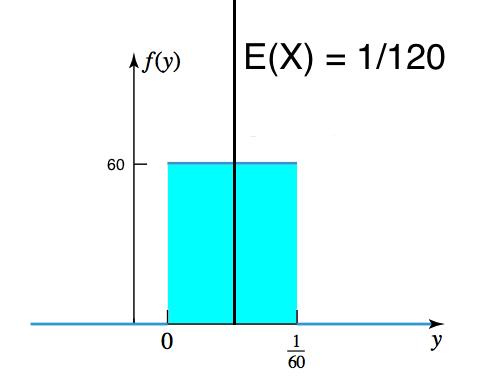
\includegraphics{../../fig/delaypictwex.png}
\end{frame}

\begin{frame}
\frametitle{Your turn: calculate E($X$)}

\begin{align*}
f(x) = \begin{cases}
0 & x < 0 \\
\frac{1}{\alpha} e^{-x/\alpha} & x \ge 0
\end{cases}
\end{align*}

\begin{enumerate}[1. ]
\item $X \sim $ Exp(3)
\item $X \sim $ Exp($\alpha$)
\end{enumerate}
\end{frame}


\begin{frame}<handout:\answers>
\frametitle{Answers: Calculate E($X$)} \scriptsize

\begin{enumerate}[1. ]

\item $X \sim $ Exp(3):
\begin{align*}
\uncover<2->{E(X)} & \uncover<2->{= \int_{-\infty}^\infty x \cdot f(x) dx} \\
&\uncover<3->{= \int_{-\infty}^0 x \cdot 0 dx + \int_{0}^\infty x \cdot \frac{1}{3} e^{-x/3} dx} \\
\intertext{\uncover<4->{integration by parts:}}
&\uncover<5->{=0 + \left (  x (-e^{-x/3})  \right)_{0}^\infty - \int_{0}^\infty (-e^{-x/3}) dx} \\
&\uncover<6->{= \left ( -\infty e^{-\infty/3} + 0 e^{-0/3} \right ) + \int_0^\infty e^{-x/3} dx} \\
&\uncover<7->{= 0 + \left ( -3e^{-x/3} \right )_0^{\infty}} \\
&\uncover<8->{= \left (-3 e^{-\infty/3} + 3 e^{-0/3} \right )} \\
&\uncover<9->{= 3}
\end{align*}
\uncover<10->{\item Similarly, E(X) = $\alpha$ when $X \sim $ Exp($\alpha$).}
\end{enumerate}
\end{frame}


\begin{frame}
\frametitle{\small Example: waiting time for the next student to arrive at the library} \scriptsize
\begin{itemize}
\pause \item From 12:00 to 12:10 PM, about 12.5 students per minute enter on average.
\pause \item Hence, the average waiting time for the next student is $\frac{1}{12.5} = 0.08$ minutes for the next student.
\pause \item Let $T \sim $ Exp($0.08$) be the time until the next student arrives.
\pause \item P(wait is more than 10 seconds) = 
\begin{align*}
\uncover<6->{P \left (T > 1/6 \right )} \uncover<7->{= 1 - F(1/6)} \uncover<8->{= 1- \left (1 - e^{(-0.08 \cdot 1/6 )} \right )} \uncover<9->{= 0.12}
\end{align*}
\setkeys{Gin}{width=.7\textwidth} \includegraphics<10->{../../fig/lib2.png}
\end{itemize}
\end{frame}

\section{Variance}

\begin{frame}
\frametitle{Variance}
\begin{itemize}
\item The variance of a continuous random variable $X$ is:
\pause \begin{align*}
\text{Var}(X) &= \int_{-\infty}^\infty (x - E(X))^2 \cdot f(x) dx 
\end{align*}
\pause Shortcut formulas:
\begin{align*}
\uncover<4->{\text{Var}(X)} & \uncover<4->{= \int_{-\infty}^\infty x^2 f(x) dx - E^2(X)} \\
&\uncover<5->{= E(X^2) - E^2(X)} \\
\end{align*}
\uncover<6->{\item The standard deviation is SD($X$) = $\sqrt{\text{Var}(X)}$}
\end{itemize}
\end{frame}


\begin{frame}
\frametitle{Your turn: checkout time}
\setkeys{Gin}{width=1\textwidth} 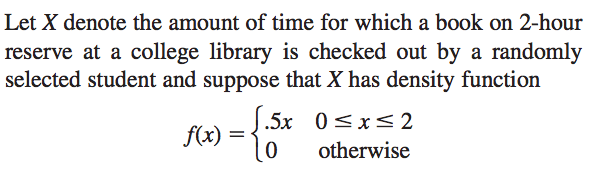
\includegraphics{../../fig/checkoutpdf.png}\q
Calculate:
\begin{enumerate}
\item E($X$)
\item Var($X$)
\end{enumerate}
\end{frame}

\begin{frame}<handout:\answers>
\frametitle{Answers: checkout time} \small
\begin{enumerate}[1. ]
\item 
\begin{align*}
E(X) &= \int_{-\infty}^\infty x \cdot f(x) dx \uncover<2->{= \int_0^2 x \cdot \frac{1}{2} x dx} \\
&\uncover<3->{= \frac{1}{2} \int_0^2 x^2 dx} \uncover<4->{= \left ( \frac{x^3}{6}\right )_0^2} \uncover<5->{ = \frac{8}{6} \approx 1.333}
\end{align*}
\uncover<6->{\item} 
\begin{align*}
\uncover<6->{E(X^2)} & \uncover<6->{= \int_{-\infty}^\infty x^2 f(x) dx} \uncover<7->{=\int_0^2 x^2 \frac{1}{2} x dx} \uncover<8->{ = \frac{1}{2} \int_{0}^2 x^3 dx} \uncover<9->{ = \left ( \frac{x^4}{8} \right )_0^2 } \\ 
&\uncover<10->{=2} \\
\uncover<11->{Var(X)} & \uncover<11->{= E(X^2) - E^2(X)} \uncover<12->{= 2 \left ( \frac{8}{6} \right ) ^2 } \\
& \uncover<13->{= \frac{2}{9}}
\end{align*}
\end{enumerate}
\end{frame}


\begin{frame}<handout:\answers>
\frametitle{Your turn: ecology}
\begin{itemize}
\item An ecologist wishes to mark off a circular sampling region having radius 10 m. However, the radius of the resulting region is actually a random variable $R$ with pdf:
\begin{center}
\begin{align*}
f(r) = \begin{cases}
\frac{3}{2} (10 - r)^2 & 9 \le r \le 11 \\
0 & \text{otherwise}
\end{cases}
\end{align*}
\end{center}
\item Calculate:
\begin{enumerate}[1. ]
\item $E(R)$
\item SD$(R)$
\end{enumerate}
\end{itemize}
\end{frame}

\begin{frame}<handout:\answers>
\frametitle{Answers: ecology} \scriptsize
\begin{enumerate}[1. ]
\item 
\begin{align*}
E(R) &= \int_{-\infty}^\infty r \cdot f(r) dr \\
&\uncover<2->{= \int_9^{11} r \cdot \frac{3}{2} (10 - r)^2 dr} \\
&\uncover<3->{= \int_{9}^{11} \left (\frac{3}{2} r^3 - 30 r^2+ 150 r \right ) dr} \\
&\uncover<4->{= \left (\frac{3}{8} r^3 - 10 r^3 + 75 r^2 \right )_9^{11}} \\
&\uncover<5->{= \left (\frac{3}{8} (11)^3 - 10 (11)^3 + 75 (11)^2 \right ) - \left (\frac{3}{8} 9^3 - 10 (9) ^3 + 75 (9)^2 \right)} \\
&\uncover<6->{= 10}
\end{align*}
\end{enumerate}
\end{frame}

\begin{frame}<handout:\answers>
\frametitle{Answers: ecology} \scriptsize
\begin{enumerate}[1. ]
\setcounter{enumi}{1}
\item 
\begin{align*}
E(R^2) &= \int_{-\infty}^\infty r^2 \cdot f(r) dr \\
&\uncover<2->{= \int_9^{11} r^2 \cdot \frac{3}{2} (10 - r)^2 dr }\\
&\uncover<3->{= \int_{9}^{11} \left (\frac{3}{2} r^4 - 30 r^3+ 150 r^2 \right ) dr} \\
&\uncover<4->{= \left (\frac{3}{10} r^5 - \frac{15}{2} r^4 + 50 r^3 \right )_9^{11}} \\
&\uncover<5->{= \left (\frac{3}{10} (11)^5 - \frac{15}{2} (11)^4 + 50 (11)^3 \right ) - \left (\frac{3}{10} (9)^5 - \frac{15}{2} (9)^4 + 50 (9)^3 \right )} \\
&\uncover<6->{= \frac{503}{5}  = 100.6} \\
\uncover<7->{\text{Var}(R)} & \uncover<7->{= E(R^2) - E^2(R)} \uncover<8->{ = \frac{503}{5} - 10^2} \uncover<9->{= \frac{3}{5} = 0.6} \\
\uncover<10->{\text{SD}(R)} & \uncover<11->{= \sqrt{\text{Var}(R)}} \uncover<12->{ = \sqrt{0.6} \approx 2.449}
\end{align*}
\end{enumerate}
\end{frame}


\section{Functions of random variables}

\begin{frame}
\frametitle{Expectation of a function of a random variable}
\begin{itemize}
\item Why does $E(X^2) = \int_{-\infty}^\infty x^2 \cdot f(x) dx$? 
\pause \item It turns out that for any function $g$ of a random variable:
\pause \begin{align*}
E(g(X)) = \int_{-\infty}^\infty g(x) \cdot f(x) dx\end{align*}
\pause \item Hence: \begin{align*}
E(X^2) = \int_{-\infty}^\infty x^2 \cdot f(x) dx
\end{align*}
if we take $g(X) = X^2$.
\pause \item In the ecology example, the expected \emph{area} of the circular sampling region is:
\pause \begin{align*}
E(\pi R^2) = \int_{-\infty}^\infty \pi r^2 \cdot f(r) dr
\end{align*}
where $\pi R^2 = g(R)$ is the sampling area.
\end{itemize}
\end{frame}

\begin{frame}
\frametitle{Expectation of a linear function of $X$} \small
\begin{itemize}
\item For constants $a$ and $b$:
\pause \begin{align*}
\uncover<2->{E(aX + b)} & \uncover<2->{= \int_{-\infty}^\infty (ax + b) \cdot f(x) dx} \\
&\uncover<3->{= a \underbrace{\int_{-\infty}^\infty x \cdot f(x) dx}_{E(X)} + b \underbrace{\int_{-\infty}^\infty f(x) dx }_{1} }\\
&\uncover<4->{= \fbox{$a E(X) + b$}}
\end{align*}
\uncover<5->{\item Example: the expected \emph{diameter} of the ecologist's sampling region is:}
\begin{align*}
\uncover<6->{E(2\cdot R + 0) = 2 \cdot E(R) + 0 = 2 \cdot 10 = 20 }
\end{align*}
\end{itemize}
\end{frame}

\begin{frame}
\frametitle{Variance of a linear function of $X$} \small
\begin{itemize}
\item For constants $a$ and $b$:
\begin{align*}
\uncover<2->{\text{Var}(aX + b)} & \uncover<2->{= E((aX + b)^2) - E^2(aX + b)} \\
&\uncover<3->{= E(a^2 X^2 + ab X + b^2) - (a E(X) + b)^2} \\
&\uncover<4->{= ( a^2 E(X^2) + ab E(X) + b^2)} \\
&\uncover<5->{ \qquad- (a^2 E^2(X) +  ab E(X) + b^2)} \\
&\uncover<6->{= a^2 (E(X^2) - E^2(X))} \\
&\uncover<7->{= \fbox{$a^2 Var(X)$}}
\end{align*}
\uncover<8->{\item Example: the variance of the \emph{diameter} of the ecologist's sampling region is:}
\begin{align*}
\uncover<9->{\text{Var}(2 \cdot R + 0) = 4 \text{Var}(R) = 4 \cdot \frac{503}{5} = \frac{2012}{5}}
\end{align*}
\end{itemize}
\end{frame}


\begin{frame}
\frametitle{Standardization} \scriptsize
\begin{itemize}
\item {\bf Standardization}: converting a random variable $X$ into another random variable $Z$ by subtracting the mean and dividing by the standard deviation:

\pause \begin{align*}
Z = \frac{X - E(X)}{SD(X)}
\end{align*}
\pause \item $Z$ has mean 0:

\begin{align*}
\uncover<4->{E(Z)} & \uncover<4->{= E \left (\frac{X - E(X)}{SD(X)} \right)} \uncover<5->{ = E \left (\frac{1}{SD(X)} \cdot X - \frac{E(X)}{SD(X)} \right )} \\
&\uncover<6->{= \frac{1}{SD(X)} \cdot E(X) - \frac{E(X)}{SD(X)}} \uncover<7->{ = 0} \\
\end{align*}

\uncover<8->{\item $Z$ has variance (and standard deviation) 1:}
\begin{align*}
\uncover<9->{\text{Var}(Z)} & \uncover<9->{= \text{Var} \left (\frac{X - E(X)}{SD(X)} \right)} \uncover<10->{ = \text{Var} \left (\frac{1}{SD(X)} \cdot X - \frac{E(X)}{SD(X)} \right)} \\
&\uncover<11->{= \frac{1}{SD^2(X)} \text{Var}(X)}  \uncover<12->{= \text{Var}(X) \frac{1}{\text{Var}(X)}} \uncover<13->{ = 1} \\
\end{align*}

\end{itemize}

\end{frame}


\end{document}
